\documentclass[revision-guide.tex]{subfiles}
%% Current Author: PS
\setcounter{chapter}{16}
\begin{document}
\raggedbottom
\chapter{Nuclear Physics}
\begin{content}
    \item equations of radioactive decay
    \item mass excess and nuclear binding energy
    \item antimatter
    \item the standard model
\end{content}
\section*{Candidates should be able to:}
\spec{show that the random nature of radioactive decay leads to the differential equation
\begin{equation} \label{n-diff} \frac{dN}{dt} = -\lambda N \end{equation} and that
\begin{equation} \label{n-exp} N = N_0 e^{-\lambda t} \end{equation} is a solution to this equation.}

Radioactive decay is characterised by the fact that the number of nuclei which disintegrate per unit time is directly proportional to the number of unchanged nuclei remaining. Since a disintegrating nucleus reduces the number remaining, there is a negative sign in the proportionality. This relationship can be expressed mathematically as equation \ref{n-diff}. Where $N$ is the number of nuclei and $\lambda$ is called the decay constant, with units \si{\per\second}.

Equation \ref{n-diff} is a differential equation with respect to time and therefore the solution to it is a function of time. We can show that equation \ref{n-exp} is a solution to this equation by differentiating it.

\begin{align*}
N &= N_0 e^{-\lambda t} \\
\frac{dN}{dt} &= \left( -\lambda \right) N_0 e^{-\lambda t} \\
&= -\lambda N
\end{align*}

\spec{recall that activity \begin{equation} A = -\frac{d N}{dt} \end{equation} and show that \( A = \lambda N \)  and \( A = A_0e^{-\lambda t}\)}

Every time a radioactive nucleus disintegrates it emits a particle of ionising radiation. Thus the activity is simply the negative of the rate of change of the number of unchanged nuclei remaining. Simple substitutions allow the derivation of the following equations.

\begin{align*}
A &= -\frac{dN}{dt} & N &= N_0 e^{-\lambda t} \\
&= -(-\lambda N) & -\lambda N &= -\lambda N_0 e^{-\lambda t} \\
&= \lambda N & A &= A_0e^{-\lambda t}
\end{align*}

Note that we do not measure the true activity as that would mean detecting all of the radiation given off by the sample. However, we assume that the measured activity is proportional to the true activity and therefore all our measurements behave in the same way.

\spec{show that the half-life \[ t_\frac{1}{2} = \frac{\ln{2}}{\lambda} \]}

The half-life is defined as the time take for half of the nuclei to decay. Therefore I can substitute $N = \frac{N_0}{2}$ into equation \ref{n-diff} to give:
\begin{align*}
\frac{1}{2} = e^{-\lambda t_\frac{1}{2}}  \\
\ln{\frac{1}{2}} = -\lambda t_\frac{1}{2} \\
t_\frac{1}{2} = \frac{\ln{2}}{\lambda}
\end{align*}

\spec{use the equations in (a), (b) and (c) to solve problems}

\spec{recognise and use the equation \begin{equation} \label{I-exp} I = I_0e^{- \mu x} \end{equation} as applied to attenuation losses}

When a wave or ionising radiation travels through a medium its amplitude will reduce due to \emph{attenuation}. This is due to scattering and/or absorption by the medium. Note that is this different to a reduction in intensity due to the radiation spreading out. It is assumed that if a given fraction of the intensity is absorbed in a unit length then eqaution \ref{n-diff} can be used, replacing $N$ with intensity, $t$ with distance, $x$ and the constant of proportionality with $\mu$. This gives
\begin{equation} \label{I-diff}
\frac{dI}{dx} = -\mu x
\end{equation}
Using a similar logic to that for equation \ref{n-exp} we can show that equation \ref{I-exp} is a solution to this equation.

\spec{recall that radiation emitted from a point source and travelling through a non-absorbing material obeys an inverse square law and use this to solve problems}

\begin{figure}[h]
  \begin{center}
    \begin{tikzpicture}[scale=0.6]
      \draw[->-, thick]  (0,0.5) -- (0,4);
      \draw[->-, thick] ({sqrt(.125)},{sqrt(.125)}) -- ({sqrt(9)},{sqrt(9)});
      \draw[->-, thick] (.5,0) -- (4,0);
      \draw[->-, thick] ({sqrt(.125)},-{sqrt(.125)}) -- ({sqrt(9)},-{sqrt(9)});
      \draw[->-, thick] (0,-.5) -- (0,-4);
      \draw[->-, thick] (-{sqrt(.125)},-{sqrt(.125)}) -- (-{sqrt(9)},-{sqrt(9)});
      \draw[->-, thick] (-.5,0) -- (-4,0);
      \draw[->-, thick] (-{sqrt(.125)},{sqrt(.125)}) -- (-{sqrt(9)},{sqrt(9)});
      \filldraw[fill=yellow] (0,0) circle (0.5cm);
    \end{tikzpicture}
  \end{center}
  \caption{Radial radiation}
  \label{radiation-spreading}
\end{figure}

Radiation emitted from a point source spreads out symmetrically in all directions as shown in figure \ref{radiation-spreading}. The intensity is defined as the power per unit area of radiation. A distance $r$ from the centre of the source the radiation is spread over the surface of a sphere and is therefore calculated using
\begin{equation}
  I = \frac{P}{4\pi r^2}
\end{equation}

Since $I\propto r^{-2}$ this is known as an inverse-square law.

\spec{estimate the size of a nucleus from the distance of closest approach of a charged particle}

When particles approach a nucleus head-on they begin with kinetic energy $E_K$. All of this kinetic energy is converted to electrical potential energy, $EPE$. If the energy of the alpha particles is known then a distance of minimum separation can be calculated.

\begin{example}
  Calculate the minimum distance of separation of a alpha particle of kinetic energy \SI{4.0}{\mega\electronvolt} travelling directly towards a gold nucleus ($Z=79$).

  \answer

  Equating the initial kinetic energy to the electrostatic potential gives
  \[ E_k = \frac{Q_1 Q_2}{4\pi \epsilon_0 d} \]
  therefore
  \begin{align*}
    d &= \frac{Q_1 Q_2}{4 \pi \epsilon_0 E_k} \\
    &= \frac{2\times79\times (\num{1.6e-19})^2}{4\pi \epsilon_0 \times \num{4.0e6} \times \num{1.6e-19}} \\
    &= \SI{5.7e-14}{\meter}
  \end{align*}
\end{example}

It turns out that if high energy alpha particles are fired at the nucleus then Rutherford's deflection formulae break down and the distribution of alpha particles no longer fits the expectation. Under these circumstances it can be assumed the alpha particle is interacting with the nucleus and therefore has been able to approach to within the nuclear radius.

\newpage
\spec{understand the concept of nuclear binding energy, and recognise and use the equation $ \Delta E = c^2 \Delta m$ (binding energy will be taken to be positive)}

It turns out that the mass of a nucleus is always smaller than the total mass of the constituent protons and neutrons. This difference is called the \emph{mass deficit} and can be converted to an energy using $ \Delta E = c^2 \Delta m$. The reduction in mass corresponds to the energy released by combining the nucleons.

\begin{example}
  Calculate the binding energy of a helium-4 nucleus of mass \SI{4.0015}{\amu}

  \answer

  The helium-4 nucleus is composed of two protons and two neutrons. Their total mass is
  \[ 2\times \SI{1.00728}{\amu}+2\times \SI{1.00867}{\amu} = \SI{4.0319}{\amu} \]
  The mass deficit, $\Delta m$, is given by
  \[ \Delta m = \SI{4.0319}{\amu} - \SI{4.00215}{\amu} = \SI{0.0304}{\amu} \]
  Therefore the binding energy is calculated as
  \[ \num{0.0304} \times \num{1.66e-27} \times c^2 = \SI{4.54e-12}{\joule} = \SI{28.4}{\mega\electronvolt} \]
\end{example}

\newpage
\spec{recall, understand and explain the curve of binding energy per nucleon against nucleon number}

A useful measure of the stability of the nucleus is given by its \emph{binding energy per nucleon}. This is the binding energy divided by the nucleon number. A plot of the binding energy per nucleon against nucleon number is show in figure \ref{binding-energy}.  The nucleus with the largest binding energy is iron-56 and this therefore is the most stable nucleus. Nuclei with nucleon numbers below iron-56 will release energy when they undergo nuclear fusion and those above iron-56 will release energy when they undergo fission.

\begin{figure}[h]
  \begin{center}
    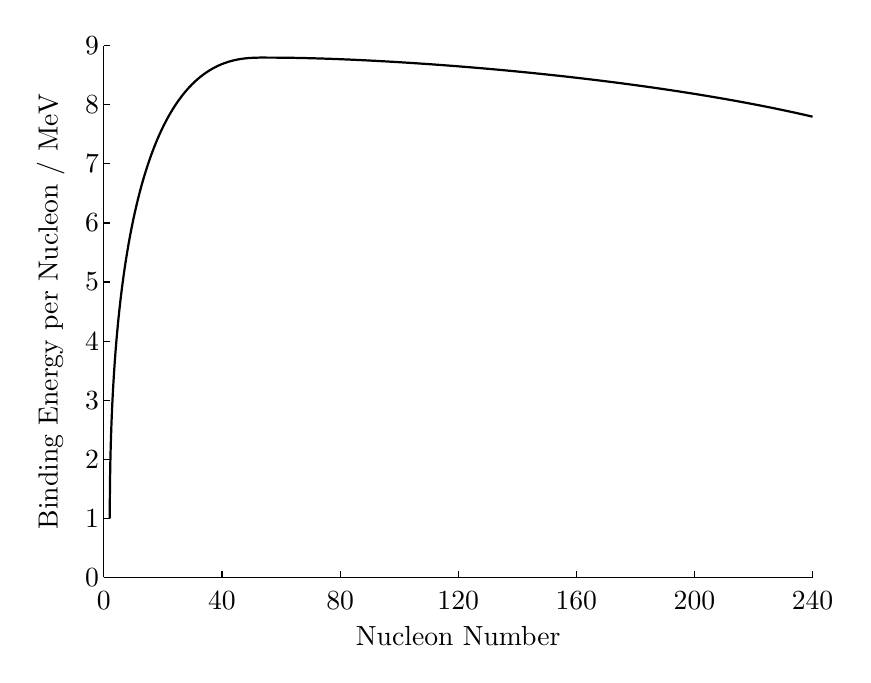
\begin{tikzpicture}[scale=0.75]
      \draw[-] (0,0) -- (0,9);
      \foreach \y in {0,1,...,9} {
        \draw (-.2,\y) node {\y};
        \draw (0,\y) -- (0.1,\y);
      }
      \draw[-] (0,0) -- (12,0);
      \foreach \x in {0,40,80,...,240} {
        \draw (\x/20,-0.4) node{{\x}};
        \draw (\x/20,0) -- (\x/20,0.1);
      }
      \draw[thick] (0.1,1) .. controls (0.1,9) and (2,8.8) .. (2.8,8.8) .. controls (4.8,8.8) and (9,8.5) .. (12,7.8);
      \draw (6,-1) node{Nucleon Number};
      \draw (-0.9,4.5) node {\rotatebox{90}{Binding Energy per Nucleon / MeV}};
    \end{tikzpicture}
  \end{center}
  \caption{Variation of binding energy per nucleon with nucleon number}
  \label{binding-energy}
\end{figure}

\spec{recall that antiparticles have the same mass but opposite charge and spin to their corresponding
particles}

All normal particles have an antiparticle partner with the same mass, but some properties which are opposite including electrical charge.

\spec{relate the equation $\Delta E = c^2 \Delta m$ to the creation or annihilation of particle-antiparticle pairs}

A particle-antiparticle pair can be created whenever there is enough energy present to do so. For example, if a photon of light is near an atomic nucleus it can spontaneously convert into an electron-positron pair.

\begin{example}
  Calculate the minimum energy a photon must have in order to create an electron-positron pair.
  \answer
  \[ E = c^2 \Delta m = c^2 \times 2 \times\num{9.11e-31} = \SI{1.02}{\mega\electronvolt} \]
\end{example}

\spec{recall the quark model of the proton (uud) and the neutron (udd)}

The theory of quarks was developed to explain the large number of particles discovered in the early particle colliders. Particles made of quarks are called \emph{hadrons}. Normal matter is made up of two types of quark, the up quark (charge $+\frac{2}{3}e$) and the down quark (charge $-\frac{1}{3}e$). From the charges it is possible to see that the proton must be uud and the neutron udd.

\spec{understand how the conservation laws for energy, momentum and charge in beta-minus decay were used to predict the existence and properties of the antineutrino}

The existence of the antineutrino was first predicted from the energy spectrum of beta decay. Beta particles are produced when a neutron in the nucleus is converted into a proton and a high energy electron. These electrons leave the nucleus at high speed and are detected as beta particles. In such a scenario (a two body process) the electrons should have a fixed amount of energy due to the conservation of momentum. However, the electron was found to have a range of energies. The explanation provided was that whenever an electron was emitted with little energy a third particle has carried away a lot of energy (and vice-versa). The particle had to be neutral (to conserve charge) and of very small mass and was named the \textbf{neutrino}.

The full beta decay equation now becomes
\[ \text{n} \rightarrow \text{p} + \text{e}^- + \overline{\nu}_\text{e} \]

Further evidence for the existence of this third particle comes from bubble chamber tracks left by beta decay which show the nucleus and electron both recoiling away from a particle which does not leave a trace in the bubble chamber - the neutrino. A photo of this decay can be seen at the science photo library here: \url{http://www.sciencephoto.com/media/1210/view}

\spec{balance nuclear transformation equations for alpha, beta-minus and beta-plus emissions}

When these nuclear decays occur total nucleon number remains the same and charge is conserved. In order to make life easier we give beta-minus particles a proton number of $-1$ and a nucleon number of zero. Beta-plus particles (positrons) are given a proton number of $+1$. Alpha particles are helium-4 nucleii ($_2^4\text{He}$).

As an example, if we know that magnesium-23 decays by beta-plus decay we can write
\[ _{12}^{23}\text{Mg} \rightarrow _Z^A\text{X} + _{1}^{0}e^+ \]

We can deduce the identity of X by conserving nucleon number ($A+0=23$) and proton number ($Z+1 = 12$). Therefore:

\[ _{12}^{23}\text{Mg} \rightarrow _{11}^{23}\text{Na} + _{1}^{0}e^+ \]

\spec{recall that the standard model classifies matter into three families: quarks (including up and down),leptons (including electrons and neutrinos) and force carriers (including photons and gluons)}

An important feature to note is that quarks and gluons are never observed on their own. There are further `generations' of quarks and leptons but these only exist at higher energies.

\spec{recall that matter is classified as baryons and leptons and that baryon numbers and lepton numbers are conserved in nuclear transformations.}

Baryons are made up of three quarks and have a baryon number of +1. Similarly, leptons have a lepton number of +1. Anti-baryons and anti-leptons have respective numbers of -1. 

For example, conservation of baryon number prohibits the following:
\begin{align*}
    p + n &\rightarrow p + e^+ + e^- \\
    B = 1 + 1 &\neq 1 + 0 + 0
\end{align*}

Conservation of lepton number also shows why the anti-electron neutrino is required in beta decay:
\begin{align*}
    n &\rightarrow p + e^- + \overline{\nu}_e \\
    L = 0 &= 0 + 1 + (-1) \\
    B = 1 &= 1 + 0 + 0
\end{align*}

\end{document}
